\chapter{Agile}

\begin{tikzpicture}[overlay,remember picture] 
\node[anchor=south] at ([yshift=5in,xshift=0.85in]current page text area.south){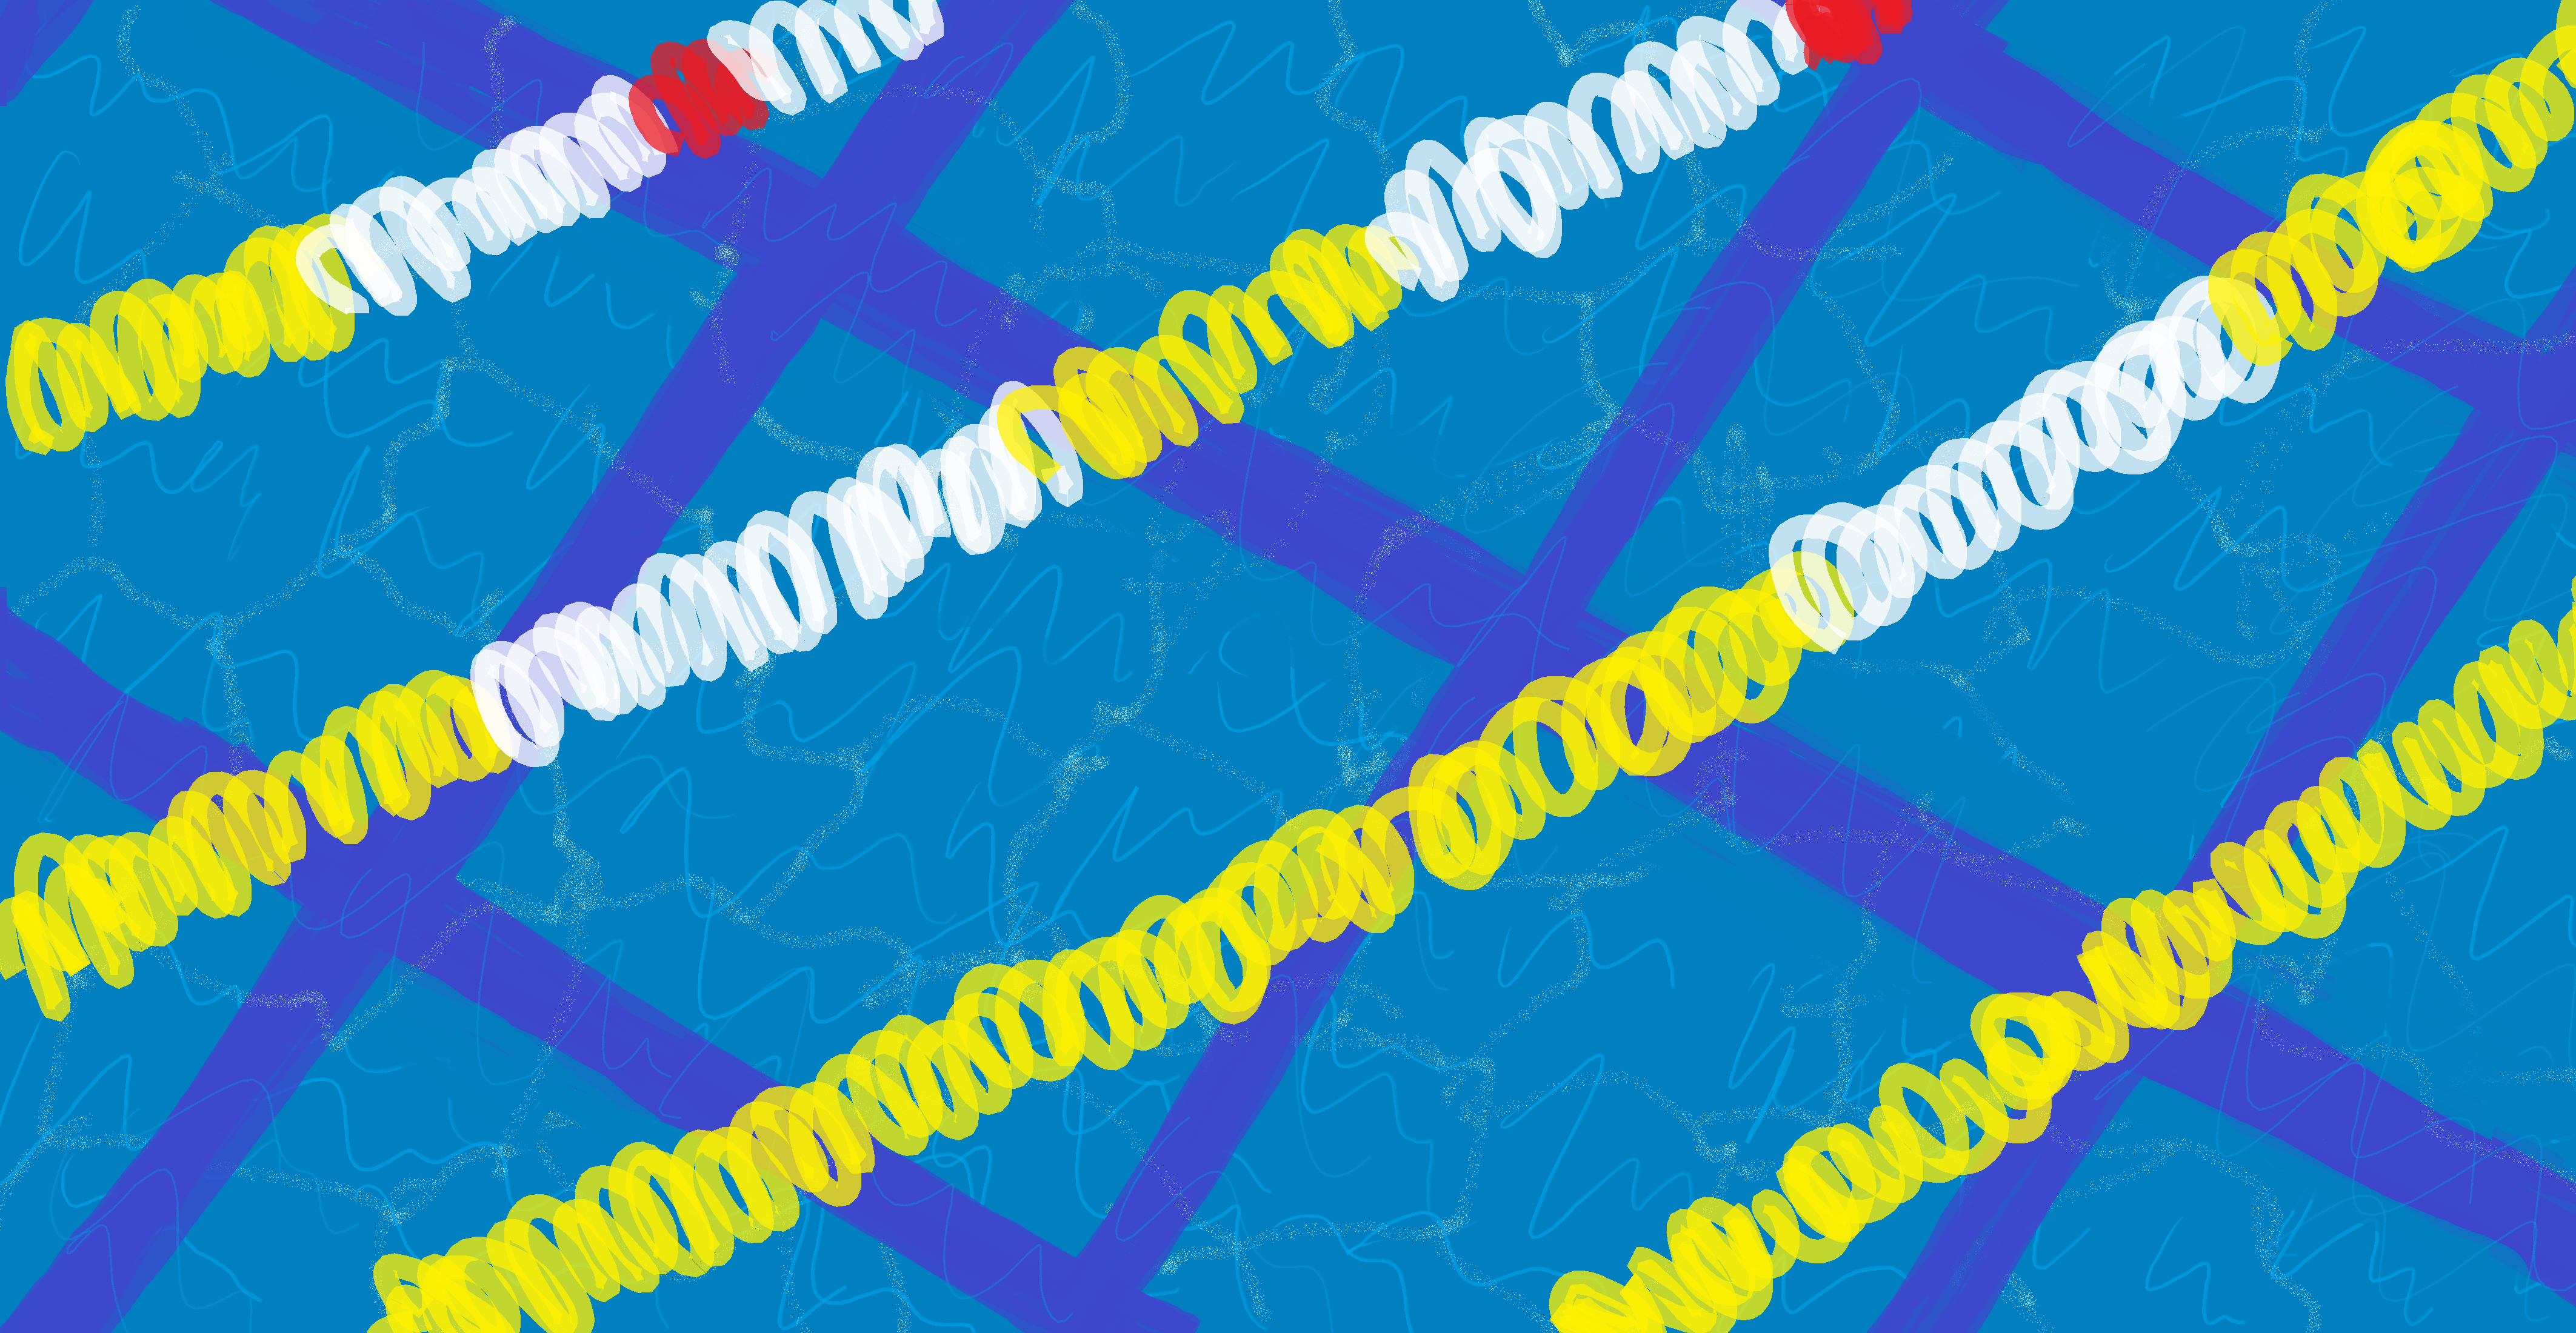
\includegraphics[width=9in]{spm04}}; 
\end{tikzpicture}

This book is geared toward \textbf{Agile}\marginpar{\agileDef\margindivider}\index{agile}, but there are other \textbf{software process models}\index{software process model}\marginpar{\softwareProcessModelDef}. Each software process model has a different way of proceeding through the \textbf{software development lifecycle (SDLC)}\index{software development lifecycle (SDLC)}. This chapter starts by describing the SDLC and Agile versus another software process model. That is followed by a discussion of \textbf{Scrum}\index{scrum} (an Agile framework) and Agile methods.

This chapter will give you the flavor of Agile and Scrum rather than being a comprehensive guide. For more detailed information about topics introduced here, see the Additional Resource section at the end of the chapter. 

\section{Software Development Lifecycle (SDLC)}

\marginpar{\scrumDef\margindivider}\marginpar{\sdlcDef\margindivider}\marginpar{\verificationDef\margindivider}\marginpar{\validationDef\margindivider}\marginpar{\maintenanceDef\margindivider}\marginpar{\incrementDef\margindivider}\marginpar{\waterfallDef}The \textbf{software development lifecycle (SDLC)}\index{software development lifecycle (SDLC)} is the way a software project proceeds through the SDLC stages: 
\begin{enumerate}
\item \textbf{Requirements}\index{requirements}: Defining what the software must do, how well it must do what it will do, and under what limitations or constraints
\item \textbf{Design}\index{design}: Defining how the code will be structured and how the user will experience the software
\item \textbf{Implementation}\index{implementation}: Coding or otherwise converting the design into a product
\item \textbf{Testing}\index{testing}: Checking that the code was written without fault (\textbf{verification}\index{verification}) and that the software is what the users or client wants (\textbf{validation}\index{validation})
\item \textbf{Maintenance}\index{maintenance}: Improving software's existing functionality
\end{enumerate}

There are different ways to travel through the SDLC stages. Patterns of travelling through the stages are called \textbf{software process models}\index{software process model}.

Commonly, people compare the Agile\index{agile} software process model with the Waterfall\index{waterfall (software process model)} model. Agile, guided by the Agile Manifesto\index{agile manifesto}, moves through the SDLC approximately like this:

\begin{center}
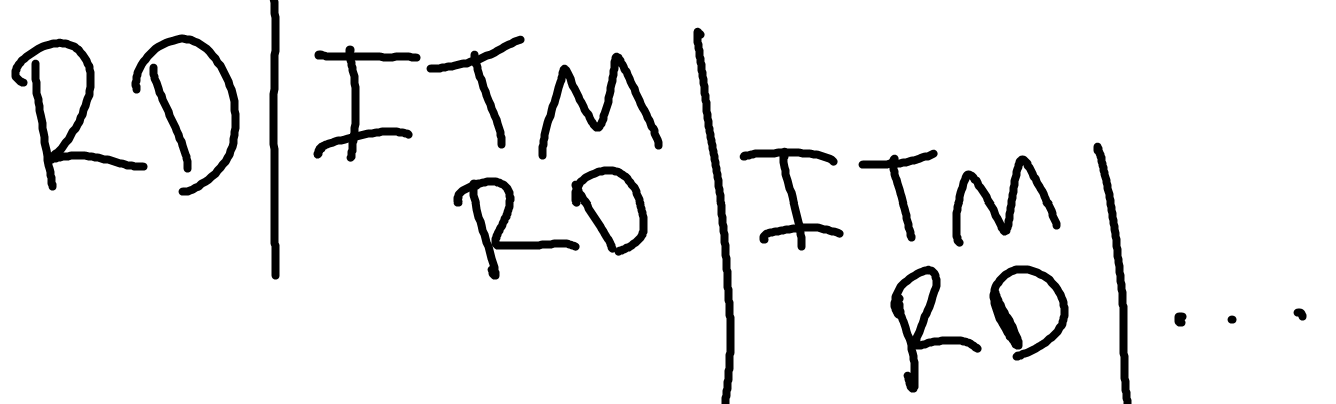
\includegraphics[width=0.8\textwidth]{agile2}
\end{center}

\textit{Vertical lines represent development cycle boundaries. Planning (R,D) for the next development cycle starts during the previous cycle.}

Agile development cycles are relatively short and numerous. Releases are frequent and \textbf{incremental}: Each cycle, there's a little more working functionality. There are multiple frameworks for developing and managing software in an Agile\index{agile} way, such as Scrum\index{scrum}, Extreme Programming (XP)\index{extreme programming (XP)}, and Kanban\index{kanban}.

\textbf{Waterfall} moves through the SDLC approximately like this:

\begin{center}
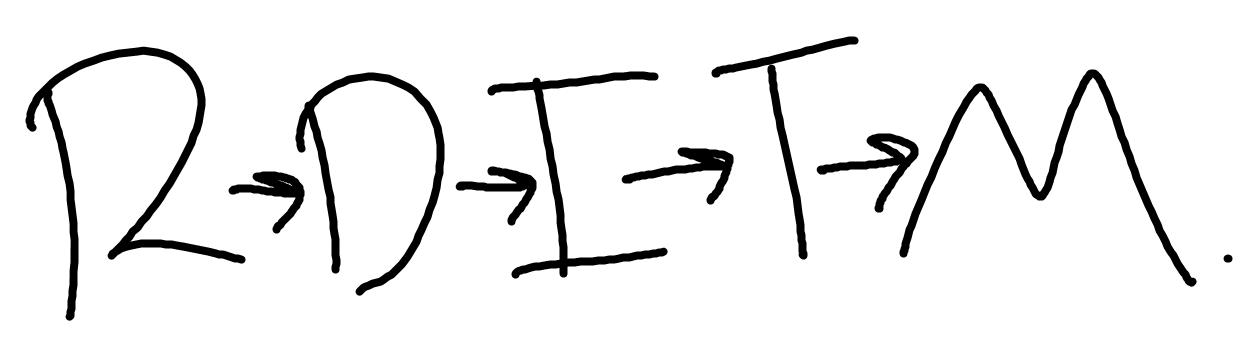
\includegraphics[width=0.8\textwidth]{waterfall}
\end{center}

Movement in linear; Each stage must be completed before moving to the next, and turning back is not allowed (you can't swim up a waterfall)---unless the project is starting over. Lots of documentation is produced on the way. There are multiple variants of Waterfall, such as the V-Model\index{v-model}, RAD\index{RAD}, and the Royce model\index{Royce model}.

\subsection{Why care about Agile, other software process models, and software engineering methods?}

\textbf{Some reasons:}\\

\begin{itemize}

\item \marginpar{The 2015 CHAOS report contains aggregate data about over 25,000 software projects.\\
\\
\textbf{Some findings about software projects}:\\
\\
56\% not on budget\\
60\% not on time\\
44\% not on target\\
43\% of ``grand'' (largest) projects failed\\
7\% of small projects failed\\
\\
\textbf{Full report}: \url{https://tinyurl.com/chaos-report-2015}
}So you can \textbf{detect and/or understand what a software development team is doing}. When you're new to a team, having a general understanding of different software process models\index{software process model} can \textbf{help you ask good questions, identify what you see the team doing, and look competent in front of your team and managers}.\\

\item So you have \textbf{ideas} to choose from when you need to select a software process model\index{software process model} or method for a \textbf{new project}. You might need to choose or recommend how your team proceeds.\\

\item So you have \textbf{ideas} to choose from when a project is \textbf{in trouble}. According to the 2015 Standish Group CHAOS Report \parencite{standish2015chaos}\index{CHAOS report}, \textbf{17 to 22\% of software projects fail}, with the likelihood of project failure \textbf{increasing drastically with project size}. Sometimes, you can save a project if you have the right methods.\\

\end{itemize}

Since this book is Agile-focused, the remainder of the chapter gives you a taste of the Agile\index{agile} software process model\index{software process model}, one Agile framework (Scrum)\index{scrum}, and a few methods that are Agile but not specifically Scrum.

\nomargins
\section{Agile, Scrum, and Agile Methods}

\subsection{Agile}

The Agile philosophy is summed up by the Agile Manifesto\index{agile manifesto} for Software Development:

\begin{displayquote}
We are uncovering better ways of developing software by doing it and helping others do it. Through this work we have come to value:
\begin{itemize}
\item \textbf{Individuals} and \textbf{interactions} over processes and tools
\item \textbf{Working software} over comprehensive documentation
\item \textbf{Customer collaboration} over contract negotiation
\item \textbf{Responding to change} over following a plan
\end{itemize}
That is, while there is value in the items on the right, we value the items on the left more.
\end{displayquote}

Why does this book have a whole chapter about Agile\index{agile} and not one about Waterfall\index{waterfall (software process model)} or any other software process model? Because most organizations use Agile\index{agile} methods for software or IT projects. For example, according to a 2017 survey by Hewlett Packard with 601 respondents, here is the distribution of what organizations use as their primary development method:

\begin{itemize}
\item 51\%: Leaning toward Agile\index{agile}
\item 46\%: Hybrid
\item 16\%: Pure Agile\index{agile}
\item 7\%: Leaning toward Waterfall\index{waterfall}
\item 2\%: Pure Waterfall\index{waterfall}
\end{itemize}

%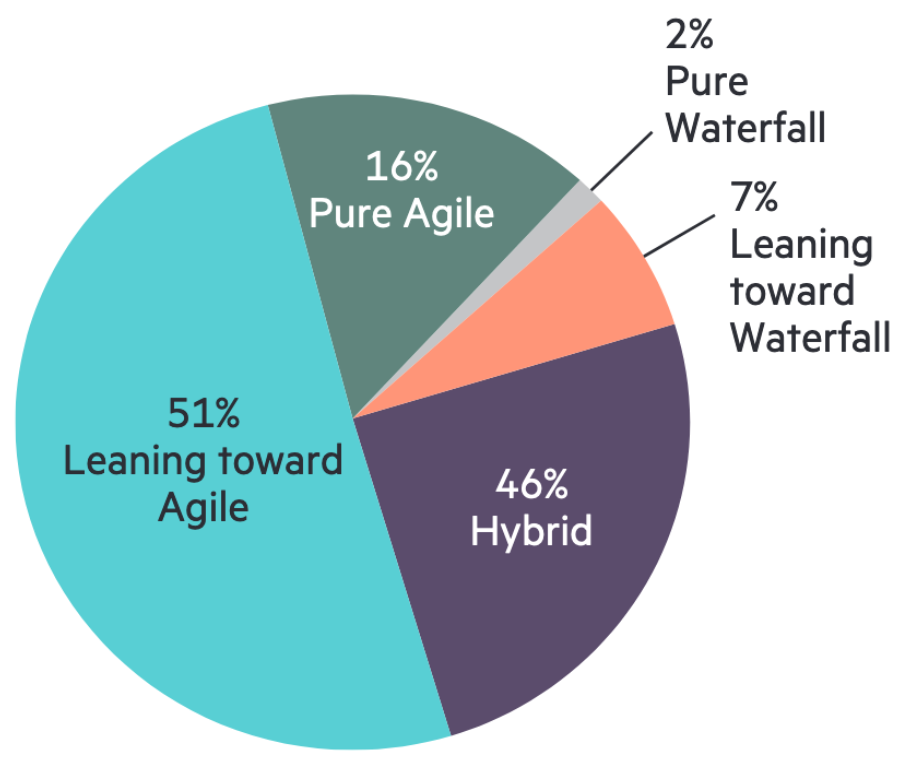
\includegraphics[scale=0.8]{agile-popularity}
%\replaceme

Why do organizations choose Agile\index{agile}? According to HP:

\spacer
\noindent Percent of respondents agreeing with statement about Agile\index{agile} development (respondents=403 organizations that have primarily adopted Agile\index{agile}):

\begin{itemize}
\item 54\%: \textbf{Enhances collaboration} between teams that don't usually work together
\item 52\%: Increases the level of \textbf{software quality} in organizations
\item 49\%: Results in increased \textbf{customer satisfaction}
\item 43\%: Shortens \textbf{time to market}
\item 42\%: Reduces \textbf{cost} of development
\end{itemize}

%\nomargins

\subsection{Scrum}

\textbf{Scrum}\index{scrum} is a set of methods that align with the Agile\index{agile} philosophy. For example, the Scrum Guide (ever-evolving manual for Scrum) \parencite{schwaber2020scrum} says that, to reflect the ``responding to change'' value, a software project should be broken into development Sprints\index{sprint} that are usually two to four weeks long. Each Sprint\index{sprint} has a Sprint Plan\index{sprint plan}. The Sprint Plan\index{sprint plan} can be defined shortly before the Sprint\index{sprint}; Teams (and their customers) might only know what they're doing for two weeks at a time.

Scrum gives teams \textbf{high-level} methods for carrying out a software development project. For example, it says nothing about how to code.

In the current version of the Scrum Guide, the methods are divided into three categories: the \textbf{team}, the \textbf{events}, and the \textbf{artifacts}. To give you a quick, convenient introduction to Scrum, the methods are listed below.

\subsubsection{The Team\index{scrum team}}

The Scrum Team\index{scrum team} ``consists of one \textbf{Scrum Master}\index{scrum master}, one \textbf{Product Owner}\index{product owner}, and \textbf{Developers}.''

\spacer
\rowcolors{2}{gray!25}{white}
\noindent\begin{tabular}{p{1.5in}|p{5in}}
\rowcolor{gray!35}
\textbf{Method (Role)} & \textbf{Definition} (Source: \href{https://www.scrumguides.org/scrum-guide.html}{The Scrum Guide})\\
Scrum Master & ``accountable for \textbf{establishing Scrum} as defined in the Scrum Guide'' \\
Product Owner\index{product owner} & ``accountable for \textbf{maximizing the value of the product} resulting from the work of the Scrum Team'' \\
Developers & ``people in the Scrum Team that are \textbf{committed to creating} any aspect of a usable Increment\index{scrum increment} each Sprint\index{sprint}''
\end{tabular}

\spacer
The Scrum Master's\index{scrum master} focus is \textbf{process}, the Product Owner's\index{product owner} focus is the \textbf{product} (software), and the Developers' focus is \textbf{creating} a product while following Scrum\index{scrum} processes.

\subsubsection{The Events\index{scrum events}}

\rowcolors{2}{gray!25}{white}
\noindent\begin{tabular}{p{1.5in}|p{5in}}
\rowcolor{gray!35}
\textbf{Method (Event)} & \textbf{Definition}\\
Sprint\index{sprint} & ``fixed length events of \textbf{one month or less} ... A new Sprint starts immediately after the conclusion of the previous Sprint'' \\
Sprint Planning\index{sprint planning} & ``initiates the Sprint by \textbf{laying out the work} to be performed'' \\
Daily Scrum\index{daily scrum} & ``a \textbf{15-minute} event for the Developers of the Scrum Team ... focuses on progress toward the Sprint Goal\index{sprint goal} and \textbf{produces an actionable plan} for the next day of work'' \\
Sprint Review\index{sprint review} & ``\textbf{to inspect} the outcome of the Sprint and determine future adaptations ... \textbf{Scrum Team and stakeholders}'' \\
Sprint Retrospective\index{sprint retrospective} & ``\textbf{to plan} ways to increase quality and effectiveness ... \textbf{Scrum Team}''
\end{tabular}

\spacer
A Sprint\index{sprint} is a development period that occurs in a series of Sprints, which are each laid out during Sprint Planning. Each day, the Developers have a ~15 minute meeting about planning the next workday. Sprints end with a Sprint Review\index{sprint review} (Team and stakeholders) and a Sprint Retrospective\index{sprint retrospective} (Team only). 

\subsubsection{The Artifacts\index{scrum artifacts}}

\rowcolors{2}{gray!25}{white}
\noindent\begin{tabular}{p{1.5in}|p{5in}}
\rowcolor{gray!35}
\textbf{Method (Artifact)} & \textbf{Definition}\\
Product Backlog\index{product backlog} & ``an emergent, \textbf{ordered list} of \textbf{what is needed} to improve the product'' \\
Sprint Backlog\index{sprint backlog} & ``composed of the \textbf{Sprint Goal}\index{sprint goal} (why), the set of \textbf{Product Backlog items selected} for the Sprint (what), as well as an \textbf{actionable plan} for delivering the Increment (how)'' \\
Increment\index{scrum increment} & ``a \textbf{concrete stepping stone} toward the Product Goal\index{product goal}''
\end{tabular}
\spacer

The Product Backlog\index{product backlog} contains a rough list of tasks the Team\index{scrum team} is planning to do sometime, but the tasks haven't yet been scheduled and may not be defined in detail. The Sprint Backlog\index{sprint backlog} contains tasks the Team has decided to work on and has added details about completing the tasks. An Increment\index{scrum increment} is an achievement toward creating the product (e.g., finishing a feature implementation).

The Scrum Guide\index{scrum guide} \parencite{schwaber2020scrum} describes the Scrum methods in more detail and defines some of the terms that were unexplained here (e.g., Sprint Goal).

\subsection{Agile Methods}

A few other Agile\index{agile} methods that aren't officially part of Scrum but are common and can be used with Scrum\index{scrum} (or other frameworks, or other software process models):

\rowcolors{2}{gray!25}{white}
\noindent\begin{tabular}{p{1.5in}|p{5in}}
\rowcolor{gray!35}
\textbf{Method} & \textbf{Description}\\
Scrum board\index{scrum board} & A way to organize and visualize tasks or work as cards on a board. The board has columns for different categories and each card is placed within a column. Could be a physical bulletin board with sticky notes or index cards. Is also a common feature of task management software.\\
Spike\index{spike} & A quick and to-the-point investigation for gathering information to help the team answer a question or choose a development path. \\
User story\index{user story} & A short description of a software feature from the perspective of fulfilling a user need (e.g, using this format: As a $<$role$>$ I can $<$capability$>$, so that $<$receive benefit$>$). Tasks, priorities, time/cost estimates, and acceptance criteria\index{acceptance criteria} may be associated with a user story.
\end{tabular}
\spacer

\section{Conclusion}
``Agile'' has associated values but no concrete meaning: It's a philosophy and there's not just one way to follow it. Agile frameworks, such as Scrum, give more concrete guidance on software development and project management. Scrum is defined by the current version of the Scrum Guide \parencite{schwaber2020scrum}, which changes frequently.

\section*{Additional Resources}

\begin{description}
    \item \fullcite{beck2000extreme}
    \item \fullcite{enterprise2017agile}
    \item \fullcite{extreme2021}
    \item \fullcite{fowler2019agile}
    \item \fullcite{royce1987managing}
    \item \fullcite{schwaber2020scrum}
    \item \fullcite{standish2015chaos}
\end{description}